% ── Experiment 16: TA vs TRE scalability, k-sweep ─────────────────────────────
% Place as a \subsubsection inside \section{Applications and experiments},
% or as part of a "Scalability" subsection --- Felix to decide cross-references.
%
% Figure: copy results/exp16_ksweep_v6_k7.pdf → paper/fig/exp16_ksweep_v6_k7.pdf
% ───────────────────────────────────────────────────────────────────────────────

\subsubsection{Scalability on nested request-grant protocols.}

We compare VolTRE against the TA-based sampler \wordgen\ \cite{wordgen} on a
parameterised family that stresses the clock-resource gap between the two
formalisms.
Consider the following $k$-level request-grant expression:
\begin{equation}\label{eq:ek}
  e_k \;=\;
  \Bigl(
    \trest{r_k \cdot
      \trest{r_{k-1} \cdot
        \trest{\cdots
          \trest{r_1 \cdot \trest{a^*g}{\leq 1}}{\leq 2}
        \cdots}{\leq k-1}
      }{\leq k}
    }{\leq k+1}
  \Bigr)^*
\end{equation}
Each cycle of $e_k$ models a protocol with $k$ request types
$r_k, r_{k-1}, \ldots, r_1$ issued in sequence,
followed by a grant $g$ within $1$ time unit of the final request $r_1$.
The nested constraints enforce cumulative deadlines: the sub-sequence
from $r_i$ must complete within $i+1$ time units.
An equivalent timed automaton requires $k$ clocks---one per deadline
level---so its state space grows exponentially in the number of clocks,
posing a scalability challenge for TA-based sampling approaches.
VolTRE, by contrast, processes each $\trest{\,\cdot\,}{\leq i}$ layer
algebraically through the slice-volume recursion, with only a
polynomial overhead per level.

\paragraph{Setup.}
We fix word length $n=10$ and vary $k=1,\ldots,7$.
For each $k$ we measure (i) the one-time preprocessing time
($t_\mathrm{vol}$ for VolTRE, $t_\mathrm{split}$ for \wordgen)
and (ii) total time including 10 samples.
\wordgen\ was given a budget of $3600$~s.
VolTRE scales to larger $n$ than shown here; we cut off where \wordgen\ fails.

\paragraph{Results.}
Figure~\ref{fig:exp16} shows total time on a logarithmic scale.
VolTRE processes all values of $k$ in well under $15$~s, with per-sample
cost growing gradually from $\approx 0.2$~s at $k{=}1$ to $\approx 5.6$~s
at $k{=}7$.
\wordgen\ is faster for small $k$ (total $\approx 1.8$~s at $k{=}5$),
but fails to terminate within the $1$~h budget at $k{=}6$ due to
memory exhaustion, and by extension for all $k\geq 6$.
This illustrates a structural advantage of the TRE representation:
the exponential blowup in the number of clocks is avoided by VolTRE's
compositional volume computation, at the cost of rejection sampling
for intersections that TA-based methods handle natively.

\begin{figure}[t]
  \centering
  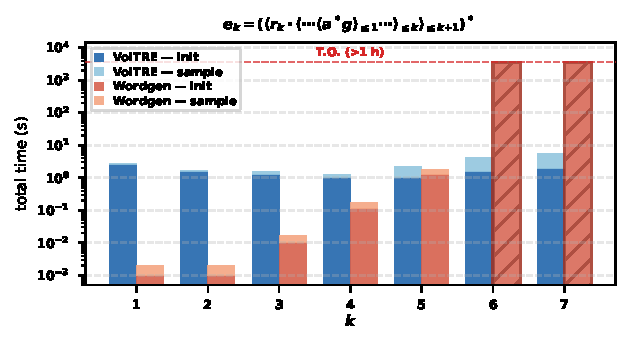
\includegraphics[width=\linewidth]{fig/exp16_ksweep_v7_k7}
  \caption{Total time (preprocessing $+$ 10 samples, log scale, $n=10$)
    for the expression family $e_k$ as $k$ varies.
    Blue: VolTRE (TRE-based).
    Red: \wordgen\ (TA-based).
    Hatched bars indicate time-out ($>\!1$~h); the dashed line marks the cutoff.}
  \label{fig:exp16}
\end{figure}
